% FAS2CriticalPathAnalysisTikZ-001
% Asset type: TikZ diagram
% Topic ID: FAS2CriticalPathAnalysis
% Purpose: Precise activity-on-arc network with durations and event-time boxes.
\documentclass[tikz,border=10pt]{standalone}
\usepackage{amsmath}
\usepackage{xcolor}
\usetikzlibrary{arrows.meta,positioning,calc}
\definecolor{Canvas}{HTML}{FAF9F6}
\definecolor{Ivory}{HTML}{FFFFF0}
\definecolor{LineSoft}{HTML}{E5E5EA}
\definecolor{AccentGold}{HTML}{D4AF37}
\definecolor{Ink}{HTML}{2C2C2E}
\begin{document}
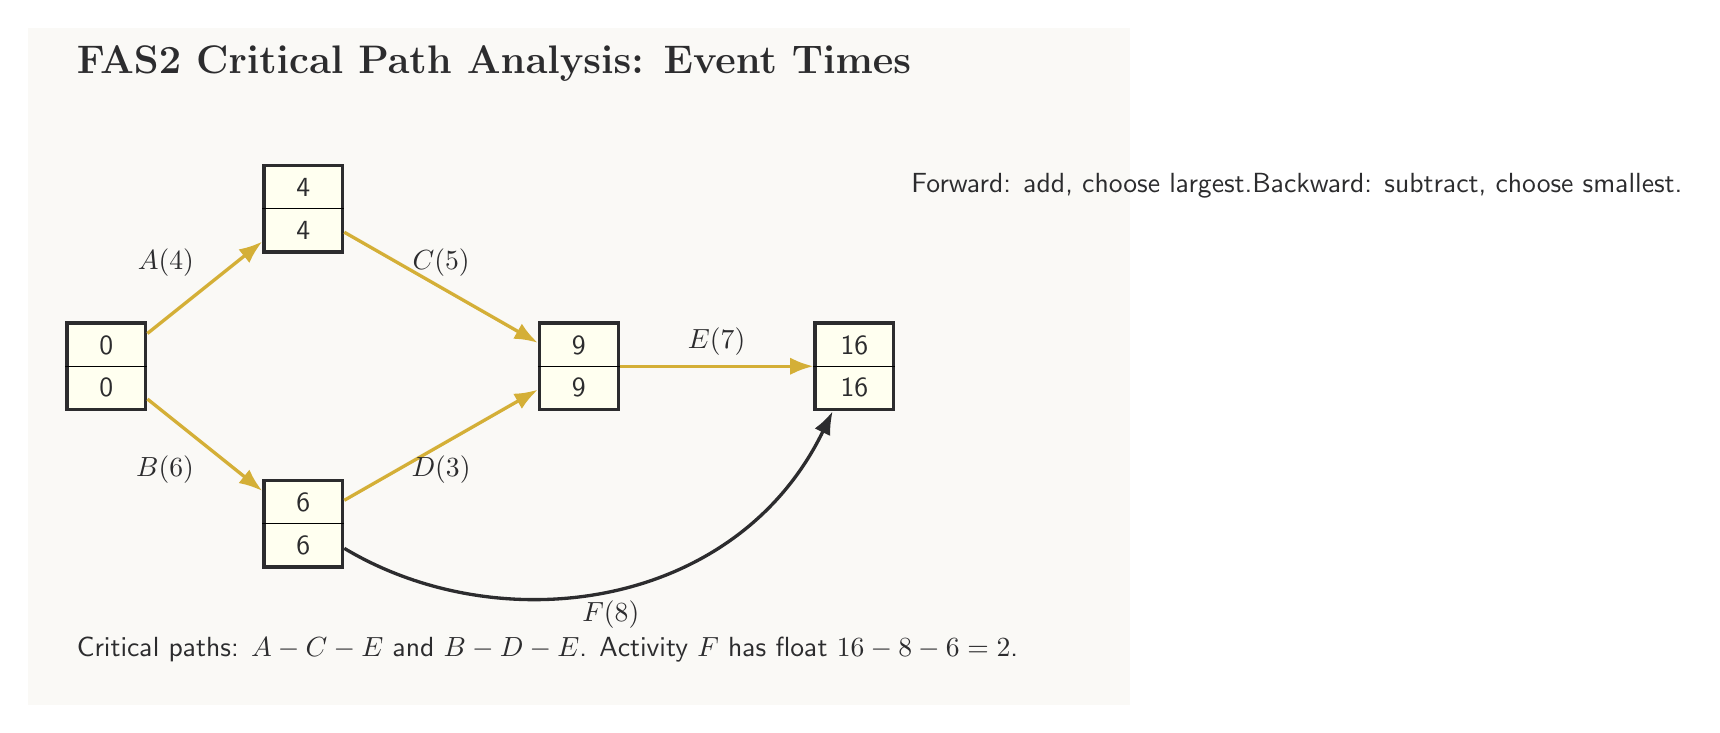
\begin{tikzpicture}[>=Latex,every node/.style={font=\sffamily,text=Ink},activity/.style={->,very thick,draw=Ink},critical/.style={->,very thick,draw=AccentGold},eventbox/.style={draw=Ink,fill=Ivory,very thick,minimum width=1cm,minimum height=1.1cm,inner sep=0pt}]
\fill[Canvas] (-1,-2.8) rectangle (13,5.8);
\node[anchor=west,font=\bfseries\Large] at (-.5,5.35){FAS2 Critical Path Analysis: Event Times};
\newcommand{\ebox}[4]{\node[eventbox](#1) at (#2){};\draw ($(#1.west)$)--($(#1.east)$);\node at ($(#1.center)+(0,.27)$){#3};\node at ($(#1.center)+(0,-.27)$){#4};}
\ebox{n0}{0,1.5}{0}{0}
\ebox{n1}{2.5,3.5}{4}{4}
\ebox{n2}{2.5,-.5}{6}{6}
\ebox{n3}{6,1.5}{9}{9}
\ebox{n4}{9.5,1.5}{16}{16}
\draw[critical](n0)--node[above left]{$A(4)$}(n1);
\draw[critical](n0)--node[below left]{$B(6)$}(n2);
\draw[critical](n1)--node[above]{$C(5)$}(n3);
\draw[critical](n2)--node[below]{$D(3)$}(n3);
\draw[critical](n3)--node[above]{$E(7)$}(n4);
\draw[activity](n2) .. controls (5,-2) and (8,-1.6) .. node[below]{$F(8)$} (n4);
\node[anchor=west] at (-.5,-2.1){Critical paths: $A-C-E$ and $B-D-E$. Activity $F$ has float $16-8-6=2$.};
\node[anchor=west] at (10.1,3.8){Forward: add, choose largest.\\Backward: subtract, choose smallest.};
\end{tikzpicture}
\end{document}
